\documentclass{article}
\usepackage{graphicx}

\begin{document}
\title{Project 3:  uniquify}
\author{Robert L. Phillips III}
\maketitle
\newpage
\tableofcontents
\newpage

\section{Design}
\subsection{Files}
\begin{enumerate}
\item parser.c/parser.h
\item merger.c/merger.h
\item main.c
\end{enumerate}

\subsection{parser.c/parser.h}
The purpose of the parser is to parse the input file.  The functionality implemented in this file directly relates to the pulling words from the input file and making sure that they are valid.  The parser was to implement four main functions.  
\\\\The first function was to simply read the next word into a buffer and return it.  The original design was to read the file character by character, but it was later determined that the same functionality could be achieved by using fscanf().  
\\\\The second function was to malloc the memory necessary to give back a new word.  
\\\\The third function was to determine if the given character was a letter or not and if it is, to convert it to lower case.
\\\\The last function was the most important function.  It was to fork and new process and then exec the sort process.  Before the sort process could be started, however, pipes must be handled.  The stdin of the newly created child process had to be overwritten with the read end of a pipe, and the stdout had to be overwritten with the write end of a pipe.  All other pipes had to be closed in the child process to ensure proper pipe management.

\subsection{merger.c/merger.h}
The purpose of the merger is to merge the words from the sort processes into one big list of unique words.  The functionality provided in this file directly relates to taking the output from each sort function in order and surpressing duplicate words and determining how many duplicates of each word are present.  
\\\\The first function was to fork the merger process.  In order for this to work correctly, the process needed access to the read end of the pipes that the sort processes would be writing to and all other pipes from the parent process needed to be closed.
\\\\The second function was to take a list of words and find the index of the word that comes first alphabetically.
\\\\The third function was to do the actual merging.  In order to merge the words, a word was taken from each pipe.  Next, the first word alphabetically had to be determined and printed out if it was different from the last word printed out.  Lastly, a new word needed to be taken from the pipe that gave the last word.  This process was repeated until all of the pipes had no more words.

\subsection{main.c}
The purpose of main is to put everything together and generate the timing statistics.  The main takes the command line argument corresponding to the number of desired processes and forks and opens the pipes necessary to perform the sort.  The words are then dealed to each of the pipes and the merge is set up.  Then process waits on its children and prints out all of the timing statistics after each child process has finished execution.

\section{Challenges}
In this assignment, the greatest challenge that I faced was knowing what pipes to close when.  It was difficult to manage all the pipes at the beginning of the assignment when I did not have a great understanding of how the pipes were being copied from parent to child.  After watching the program execute step by step, it became clear what pipes were being copied when and how they needed to be managed.  Another problem I ran into was foregetting to wait for the merger process in the parent.  This led to the issue of the program terminating before the merge process finished, which, at first glance, made it appear as if the program was still running because the terminal prompt would not show up after the merger finished writing to stdout.

\section{Work Log}
\begin{enumerate}
\item \textbf{Revision 1} (Wed 31 Oct 2012 10:12 AM) 0.8 hours:  Implemented the function to read through a text file word by word.  Also wrote the loop to iterate through the file word by word so that it can later pass the words out in a deck of cards fashion.
\item \textbf{Revision 2} (Thu 1 Nov 2012 8:31 AM) 2.9 hours:  Wrote the function that forked all of the sort processes and passes the words in a text file to the sort processes.  For the time being, the output of the sort processes were left on stdout so the output of the sort functions could be manually verified.
\item \textbf{Revision 3} (Thu 1 Nov 2012 7:22 PM) 1.5 hours:  Redirected the output of the sort functions to the pipes associated with the merger process.
\item \textbf{Revision 4} (Fri 2 Nov 2012 12:11 PM) 2.4 hours:  Wrote the code to merge the output of the sort process and print it to stdout.  Found a bug that makes it appear as if the program is still running, which happens at different times throughout the program execution.
\item \textbf{Revision 5} (Sat 3 Nov 2012 7:57 PM) 2.1 hours:  Found the source of the R4 bug and fixed it.  Wrote the functions to print out the timing info.  Combined all the functions to create the finished program.  
\item \textbf{Revision 6} (Sun 4 Nov 2012 11:47 AM) 1.6 hours:  Began generating
 output for the graphs and working on the write-up.
\item\textbf{Revision 7} (Mon 5 Nov 2012 10:10 AM) 0.9 hours:  Finished the timing graphs and imported them into the \LaTeX{} file to be turned in.

\end{enumerate}

\section{Timings}
\makebox[\textwidth]{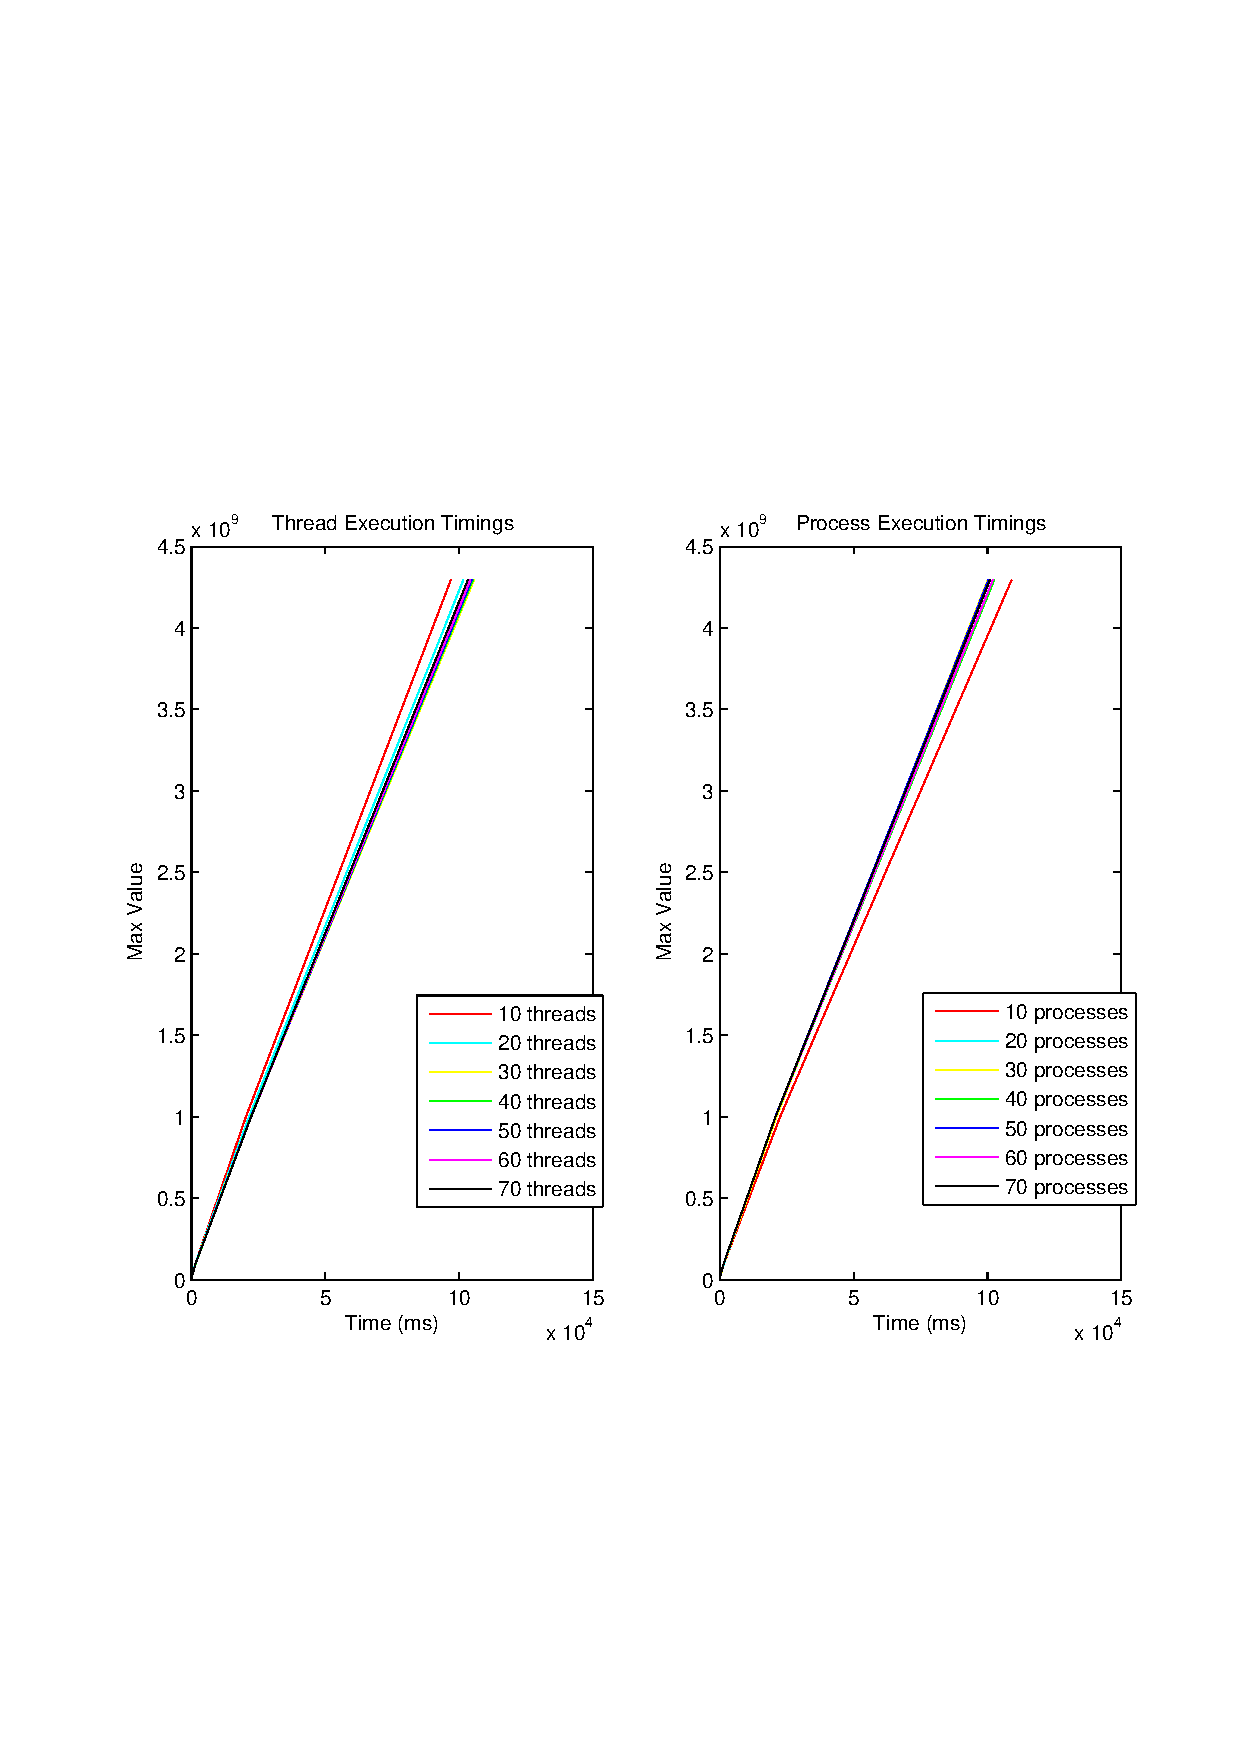
\includegraphics[width=\textwidth]{timing.pdf}}

\section{Additional Questions}
\begin{enumerate}
\item I believe the main point of this assignment was to get comfortable using pipes and concepts related to parallel programming.  Another purpose of this assignment is to get familiar how memory is copied between child processes and parents processes at the time of creation.
\item In order to verify my solution was correct, I isolated the three separate parts of the program from each other.  I started by writing a parser.  I took several small text files and manually verified that the output of my parser was correct by comparing the output sent to the terminal with contents of each text file.  Once the parser was working, the sort processes needed to be coded and tested.  The testing of the sort processes was done in the same fashion as the parser.  The output of each of the sort processes was manually inspected to make sure that each of the processes had the same number of words (or 1 more) and that each of the subsets of words was sorted correctly.  Once the first two were functioning correctly, the merger needed to be coded and tested.  It was tested in the same way.  The merger was tested on several small data sets before it was tested with larger words lists.
\item I learned that pipes and child processes need to be managed carefully in order for parallel programming to be done correctly.  I also learned that fscanf() is really useful for reading in files word by word.  The most important thing that I learned is how to use pipes for inter process communication.
\end{enumerate}

\end{document}
